\documentclass[a4paper]{article}
\usepackage{a4wide,amssymb,epsfig,latexsym,multicol,array,hhline,fancyhdr}
\usepackage[utf8]{vietnam}
\usepackage[vietnamese,english]{babel}
\usepackage{amsmath}
\usepackage{lastpage}
\usepackage[lined,boxed,commentsnumbered]{algorithm2e}
\usepackage{enumerate}
\usepackage{color}
\parindent 0pt
\usepackage{graphicx}							% Standard graphics package
\usepackage{array}
\usepackage{float}
\usepackage{tabularx, caption}
\usepackage{multirow}
\usepackage{multicol}
\usepackage{rotating}
\usepackage{graphics}
\usepackage{geometry}
\usepackage{setspace}
\usepackage{epsfig}
\usepackage{listings}
\usepackage{tikz}
\usetikzlibrary{arrows,snakes,backgrounds}
\usepackage{hyperref}
\hypersetup{urlcolor=blue,linkcolor=black,citecolor=black,colorlinks=true} 
%\usepackage{pstcol} 								% PSTricks with the standard color package

\usepackage{xcolor}
\definecolor{codegreen}{rgb}{0,0.6,0}
\definecolor{codegray}{rgb}{0.5,0.5,0.5}
\definecolor{codepurple}{rgb}{0.58,0,0.82}
\definecolor{backcolour}{rgb}{0.95,0.95,0.92}

\lstdefinestyle{mystyle}{
    backgroundcolor=\color{backcolour},   
    commentstyle=\color{codegreen},
    keywordstyle=\color{magenta},
    numberstyle=\tiny\color{codegray},
    stringstyle=\color{codepurple},
    basicstyle=\ttfamily\footnotesize,
    breakatwhitespace=false,         
    breaklines=true,                 
    captionpos=b,                    
    keepspaces=true,                 
    numbers=left,                    
    numbersep=5pt,                  
    showspaces=false,                
    showstringspaces=false,
    showtabs=false,                  
    tabsize=2
}
\lstset{style=mystyle}

\newtheorem{theorem}{{\bf Theorem}}
\newtheorem{property}{{\bf Property}}
\newtheorem{proposition}{{\bf Proposition}}
\newtheorem{corollary}[proposition]{{\bf Corollary}}
\newtheorem{lemma}[proposition]{{\bf Lemma}}

\AtBeginDocument{\renewcommand*\contentsname{Contents}}
\AtBeginDocument{\renewcommand*\refname{References}}
%\usepackage{fancyhdr}
\setlength{\headheight}{40pt}
\pagestyle{fancy}
\fancyhead{} % clear all header fields
\fancyhead[L]{
 \begin{tabular}{rl}
    \begin{picture}(25,15)(0,0)
    \put(0,-8){
\includegraphics[width=8mm, height=8mm]{graphics/hcmut.png}}
    %\put(0,-8){\epsfig{width=10mm,figure=hcmut.eps}}
   \end{picture}&
	%
\includegraphics[width=8mm, height=8mm]{hcmut.png} & %
	\begin{tabular}{l}
		\textbf{\bf \ttfamily University of Technology, Ho Chi Minh City}\\
		\textbf{\bf \ttfamily Faculty of Applied Science}
	\end{tabular} 	
 \end{tabular}
}
\fancyhead[R]{
	\begin{tabular}{l}
		\tiny \bf \\
		\tiny \bf 
	\end{tabular}  }
\fancyfoot{} % clear all footer fields
\fancyfoot[L]{\scriptsize \ttfamily Assignment for Probability \& Staticstics - Academic year 2024}
\fancyfoot[R]{\scriptsize \ttfamily Page {\thepage}/\pageref{LastPage}}
\renewcommand{\headrulewidth}{0.3pt}
\renewcommand{\footrulewidth}{0.3pt}


%%%
\setcounter{secnumdepth}{4}
\setcounter{tocdepth}{3}
\makeatletter
\newcounter {subsubsubsection}[subsubsection]
\renewcommand\thesubsubsubsection{\thesubsubsection .\@alph\c@subsubsubsection}
\newcommand\subsubsubsection{\@startsection{subsubsubsection}{4}{\z@}%
                                     {-3.25ex\@plus -1ex \@minus -.2ex}%
                                     {1.5ex \@plus .2ex}%
                                     {\normalfont\normalsize\bfseries}}
\newcommand*\l@subsubsubsection{\@dottedtocline{3}{10.0em}{4.1em}}
\newcommand*{\subsubsubsectionmark}[1]{}
\makeatother


\begin{document}

\begin{titlepage}
\begin{center}
VIETNAM NATIONAL UNIVERSITY, HO CHI MINH CITY \\
UNIVERSITY OF TECHNOLOGY \\
FACULTY OF APPLIED SCIENCE
\end{center}

\vspace{1cm}

\begin{figure}[h!]
\begin{center}

\includegraphics[width=3cm]{graphics/hcmut.png}
\end{center}
\end{figure}

\vspace{1cm}


\begin{center}
\begin{tabular}{c}
\multicolumn{1}{l}{\textbf{{\Large PROBABILITY \& STATISTICS (MT2013)}}}\\
~~\\
\hline
\\
\multicolumn{1}{l}{\textbf{{Semester: 231}}}\\
\\
\textbf{{\Huge Central Processing Units (CPUs)}}\\
\\
% \textbf{{\Huge (chwa biet ghi gi)}}\\[10pt]

\multicolumn{1}{l}{\textbf{{}}}\\
\\
\hline
\end{tabular}
\end{center}

\vspace{2cm}

\begin{table}[h]
	\begin{tabular}{rrl}
		\hspace{5 cm} & Advisor: & Phan Thị Khánh Vân,\hspace*{10pt} FAS - HCMUT\\[6pt]
		& Students: & Lê Nguyễn Gia Bảo \hspace*{12pt} - 2210216. \\
		& 			& Trần Đình Đăng Khoa \hspace*{0pt} - 2211649. \\
		& 			& Bùi Vũ Thiên Đăng	  \hspace*{13pt} - 2252151. \\
		& 			& Trần Tuấn Minh Khoa 	  \hspace*{0pt} - 2252365. \\
		& 			& Nguyễn Hữu Trí		  \hspace*{28pt} - 2252842. \\
	\end{tabular}
\end{table}

\vspace*{1cm}

\begin{center}
{\footnotesize HO CHI MINH CITY, APRIL 2024}
\end{center}
\end{titlepage}

%\thispagestyle{empty}

\newpage
\tableofcontents

% %%%%%%%%%%%%%%%%%%%%%%%%%%%%%%%%%
% \section{Member list \& Workload}

\begin{center}
\begin{tabular}{|c|c|c|c|}
\hline
\textbf{No.} & \textbf{Fullname} & \textbf{Student ID} & \textbf{Contribution}\\
\hline 
%%%%%Student 1%%%%%%%%%%
\multirow{1}{*}{1} & \multirow{1}{*}{Lê Nguyễn Gia Bảo} & \multirow{1}{*}{2210216} & \multirow{1}{*}{20\%}\\
\hline 
%%%%%Student 2%%%%%%%%%%%
\multirow{1}{*}{2} & \multirow{1}{*}{Trần Đình Đăng Khoa} & \multirow{1}{*}{2211649} & \multirow{1}{*}{20\%}\\
\hline
%%%%%Student 3%%%%%%%%%%%
\multirow{1}{*}{3} & \multirow{1}{*}{Bùi Vũ Thiên Đăng} & \multirow{1}{*}{2252151} & \multirow{1}{*}{20\%}\\
%%%%%Student 4%%%%%%%%%%%
\hline
\multirow{1}{*}{4} & \multirow{1}{*}{Trần Tuấn Minh Khoa} & \multirow{1}{*}{2252365} & \multirow{1}{*}{20\%}\\
%%%%%Student 5%%%%%%%%%%%
\hline
\multirow{1}{*}{5} & \multirow{1}{*}{Nguyễn Hữu Trí} & \multirow{1}{*}{2252842} & \multirow{1}{*}{20\%}\\
\hline
\end{tabular}
\end{center}
% %%%%%%%%%%%%%%%%%%%%%%%%%%%%%%%%%
% \section{Abstract}

In the rapidly advancing field of computer hardware technology, understanding and predicting the clock speed (frequency) of central processing units (CPUs) is crucial for both manufacturers and consumers. This project, \textbf{"Predicting Intel CPU Clock Speed Using Statistical Methods"}, aims to develop robust predictive models for CPU clock speed based on detailed specifications of Intel CPUs. By employing statistical techniques such as \textbf{Linear Regression} and \textbf{Analysis of Variance (ANOVA)}, this study seeks to identify the key features that significantly influence CPU clock speed.\\

The dataset utilized in this study comprises a comprehensive collection of Intel CPU specifications, including attributes such as the number of cores, number of threads, cache size, power consumption, and various architectural details. Data preprocessing steps involve handling missing values, normalizing data, and encoding categorical variables to ensure the dataset is suitable for rigorous statistical analysis.\\

To identify significant predictors of CPU clock speed, ANOVA is used to assess the impact of categorical variables, providing insights into how different CPU series and generations affect clock speeds. Linear regression is then employed to model and predict CPU clock speed based on these significant features. This method directly establishes the relationship between the dependent variable (clock speed) and the independent variables (CPU specifications).\\

The predictive modeling component of this project primarily relies on linear regression techniques. Linear regression provides a foundational understanding of the linear relationships between the predictors and CPU clock speed. The performance of the regression models is evaluated using key metrics such as R-squared, Mean Squared Error (MSE), and visual inspection of residual plots.\\

Our analysis reveals that features such as the number of cores, number of threads, cache size, and power consumption are significant determinants of CPU clock speed. The linear regression model offers valuable insights into the impact of these features on clock speed, allowing for accurate predictions based on the given specifications. While ANOVA provides supplementary information on the influence of categorical variables, it is the linear regression model that forms the core of our predictive analysis.\\

This project contributes to the broader understanding of CPU performance dynamics, providing a methodological framework that can be applied to other hardware components or similar predictive tasks. The findings have practical implications for manufacturers in optimizing CPU design and for consumers in making informed purchasing decisions. By leveraging statistical methods and regression analysis, this study offers a data-driven approach to predicting CPU clock speed, enhancing transparency and efficiency in the marketplace.\\


\newpage
% %%%%%%%%%%%%%%%%%%%%%%%%%%%%%%%%%
\section{Introduction}

The Central Processing Unit (CPU) is often referred to as the "brain" of the computer due to its fundamental role in executing instructions and managing the operations of other components. It processes data, performs calculations, and manages tasks, making it a critical component that directly impacts a computer's performance and efficiency. As technology continues to advance rapidly, the variety and complexity of CPUs available in the market have also increased, necessitating more sophisticated methods to evaluate and predict their clock speed (frequency).\\

Predicting CPU clock speed accurately is crucial for several reasons. For manufacturers, understanding the factors that influence CPU clock speed can aid in optimizing CPU design, enhancing product development, and targeting the right market segments. Accurate clock speed predictions can help manufacturers maintain a balance between performance and cost-effectiveness. For consumers, knowledge of CPU performance dynamics enables informed purchasing decisions, ensuring that they obtain the best value for their money. This is particularly important given the diverse range of CPUs available, each with different specifications and performance levels.\\

This report focuses on the analysis of CPU specifications to predict clock speed using a variety of statistical methods. The dataset used in this study consists of detailed specifications of Intel CPUs, one of the leading CPU manufacturers in the world. Intel CPUs are widely used in various computing devices, from desktops and laptops to servers and workstations, making them an ideal subject for this study.\\

The primary goal of this report is to identify the key features that significantly influence CPU clock speed and to develop predictive models that can accurately estimate clock speeds based on the identified features. To achieve this, we employ several statistical techniques, including Analysis of Variance (ANOVA) and regression analysis. Each of these methods plays a vital role in understanding the relationships between different CPU specifications and their corresponding clock speeds.\\

Analysis of Variance (ANOVA) is utilized to determine the impact of categorical variables on CPU clock speed. By comparing means across different groups, ANOVA helps identify whether certain categorical features, such as CPU series or generation, significantly affect clock speed. This analysis provides supplementary insights that enhance our understanding of how different CPU models and architectures impact performance.\\

The regression analysis forms the core of our predictive modeling approach. Linear regression is applied to provide a foundational understanding of the linear relationships between the selected features and CPU clock speed. Given the complexity of CPU performance, we also consider polynomial regression to capture potential non-linear interactions among the variables. By comparing the performance metrics of these models, such as R-squared and Mean Squared Error (MSE), we can determine the most effective model for predicting CPU clock speed.\\

Data preprocessing is a crucial step in this analysis, ensuring the reliability and accuracy of our models. This involves handling missing values, normalizing data, and encoding categorical variables. Proper preprocessing enhances the quality of the dataset, making it suitable for rigorous statistical analysis and modeling.\\

In summary, this report aims to provide a comprehensive analysis of Intel CPU specifications to predict their clock speeds. By leveraging statistical methods and regression models, we seek to develop robust predictive models that can assist manufacturers in optimizing CPU design and help consumers make informed purchasing decisions. The findings of this study will contribute to the broader understanding of CPU performance dynamics and demonstrate the value of combining various statistical techniques to create accurate and reliable clock speed predictions.\\

\newpage
% %%%%%%%%%%%%%%%%%%%%%%%%%%%%%%%%%
\section{Background Knowledge}
\subsection{Hypothesis Testing}
Hypothesis testing is a fundamental statistical procedure used to make inferences about population parameters based on sample data. It is widely employed in various fields, including scientific research, quality control, and decision-making processes. The primary objective of hypothesis testing is to evaluate the plausibility of a specific claim or hypothesis concerning a population parameter, such as the mean, proportion, or variance.\\

In hypothesis testing, two mutually exclusive hypotheses are formulated: the null hypothesis ($H_0$) and the alternative hypothesis ($H_a$). The null hypothesis typically represents the status quo, the baseline assumption, or the claim that the researcher wishes to test against. The alternative hypothesis represents the opposite or the alternative claim that the researcher aims to support or conclude if the null hypothesis is rejected.\\

The process of hypothesis testing involves the following steps:
\begin{enumerate}
    \item Formulate the null hypothesis ($H_0$) and the alternative hypothesis ($H_a$).
    \item Specify the significance level ($\alpha$), which is the probability of rejecting the null hypothesis when it is true (Type I error).
    \item Calculate the test statistic from the sample data.
    \item Determine the critical region or the critical value(s) based on the significance level and the chosen test.
    \item Compare the test statistic with the critical region or critical value(s).
    \item Make a decision: Reject or fail to reject the null hypothesis.
\end{enumerate}

The decision to reject or fail to reject the null hypothesis is based on the comparison between the test statistic and the critical region or critical value(s). If the test statistic falls within the critical region, the null hypothesis is rejected in favor of the alternative hypothesis. If the test statistic does not fall within the critical region, the null hypothesis is not rejected.\\

There are several types of hypothesis tests, including:
\begin{itemize}
    \item Tests for means (one-sample, two-sample, and paired data)
    \item Tests for proportions
    \item Tests for variances
    \item Tests for correlation and regression coefficients
    \item Goodness-of-fit tests
    \item Non-parametric tests
\end{itemize}
The choice of the appropriate hypothesis test depends on the nature of the data, the research question, and the assumptions underlying the statistical model.\\

It is important to note that hypothesis testing is subject to two types of errors: Type I error (rejecting the null hypothesis when it is true) and Type II error (failing to reject the null hypothesis when it is false). The significance level ($\alpha$) controls the probability of committing a Type I error, while the power of the test (1 - $\beta$) represents the probability of correctly rejecting the null hypothesis when it is false, where $\beta$ is the probability of committing a Type II error.\\

Hypothesis testing is a powerful tool for making statistical inferences and drawing conclusions from data. However, it is crucial to carefully interpret the results, consider the practical implications, and recognize the limitations and assumptions underlying the chosen statistical test.

\subsection{Linear Regression}
Linear regression is a fundamental statistical technique used to model the relationship between a dependent variable and one or more independent variables. It is widely employed in various fields, including economics, finance, engineering, and social sciences, to analyze and make predictions based on observed data.\\

The primary objective of linear regression is to find the best-fitting straight line that describes the relationship between the dependent variable (also known as the response variable) and the independent variable(s) (also known as predictor variables or explanatory variables). This line is represented by a linear equation, which takes the following form:
$$ Y = \beta_0 + \beta_1x_1 + \beta_2x_2 + ... + \beta_nx_n + \varepsilon  $$
Where:
\begin{itemize}
    \item Y is the dependent variable
    \item $ \beta_0 $ is the intercept (the value of y when all independent variables are zero)
    \item $ \beta_1,  \beta_2, ...,  \beta_n$ are the coefficients (slopes) associated with the respective independent variables
    \item $x_1, x_2, ..., x_n$ are the independent variables
    \item $\varepsilon$ is the error term, representing the difference between the observed values and the predicted values
\end{itemize}

\vspace*{1cm}

The process of linear regression involves estimating the values of the coefficients ($\beta_0$, $\beta_1$, $\beta_2$, ..., $\beta_n$) using a set of observed data points. This estimation is typically performed using the method of least squares, which aims to minimize the sum of squared differences between the observed values and the predicted values obtained from the linear equation.
Linear regression models can be classified into two main types:

\begin{itemize}
    \item Simple Linear Regression: This model involves only one independent variable and is represented by the equation $ Y = \beta_0 + \beta_1x + \varepsilon  $.
    \item Multiple Linear Regression: This model involves two or more independent variables and is represented by the equation $ Y = \beta_0 + \beta_1x_1 + \beta_2x_2 + ... + \beta_nx_n + \varepsilon  $
\end{itemize}

Once the linear regression model is fitted to the data, it can be used for various purposes, such as:

\begin{enumerate}
    \item Prediction: The model can be used to predict the value of the dependent variable based on new values of the independent variables.
    \item Inference: Statistical tests can be performed to assess the significance of the independent variables and the overall model fit.
    \item Interpretation: The coefficients of the independent variables can be interpreted to understand the magnitude and direction of their impact on the dependent variable.
\end{enumerate}

It is important to note that linear regression models make several assumptions, including linearity, normality of residuals, homoscedasticity (constant variance of residuals), and independence of observations. Violations of these assumptions can lead to biased or inefficient estimates and invalid statistical inferences.\\

Additionally, linear regression models are susceptible to issues such as multicollinearity (high correlation among independent variables) and outliers, which can influence the model's performance and interpretability. Various diagnostic techniques and model validation methods are employed to assess the reliability and robustness of the linear regression model.\\

Linear regression serves as a foundation for more advanced regression techniques, such as logistic regression (for binary or categorical dependent variables), nonlinear regression, and time series analysis, among others. Its simplicity, interpretability, and widespread applicability make linear regression a fundamental tool in statistical modeling and data analysis.

\newpage
% %%%%%%%%%%%%%%%%%%%%%%%%%%%%%%%%%
\section{Data Pre-processing}
\subsection{Load Data}
\begin{lstlisting}[language=R]
    # Importing data 
    intel_cpu <- read.csv ("~/Downloads/archive/Intel_CPUs.csv")
\end{lstlisting}

This line of R code is used to import a dataset from a Comma-Separated Values (CSV) file into the R environment.
The \texttt{read.csv()} function is a built-in function in R that reads a CSV file and creates a data frame object from its contents. A data frame is a two-dimensional tabular data structure in \texttt{R}, where each column represents a variable, and each row represents an observation.\\

In this specific code:
"\textbf{$\sim$/Downloads/archive/Intel\_CPUs.csv}" is the file path that specifies the location and name of the CSV file to be imported, \texttt{intel\_cpu} is the name assigned to the data frame object that will store the imported data.\\

After executing this line of code, the contents of the "\textbf{Intel\_CPUs.csv}" file will be read and stored in the \texttt{intel\_cpu} data frame within the \texttt{R} environment. The data frame will have the same structure as the CSV file, with columns representing variables and rows representing observations.

\subsection{Explore Data}
\begin{lstlisting}[language=R]
    # The head () function is used to preview the first 
    # few rows of the data frame
    head (intel_cpu)
\end{lstlisting}

This line calls the \texttt{head()} function and passes the \texttt{intel\_cpu} data frame as an argument. By default, the \texttt{head()} function prints the first \textit{six} rows of the given data frame or matrix.\\

The \texttt{head()} function is a valuable tool for data exploration and validation, especially when working with large datasets. By previewing the initial rows, you can quickly assess the structure of the data, check the column names, and ensure that the data has been imported correctly.\\

Inspecting the first few rows can reveal potential issues or anomalies in the data, such as missing values, incorrect data types, or unexpected values. It also provides an initial glimpse into the content and format of the data, which can inform subsequent data cleaning, transformation, or analysis steps

\begin{figure}[H]
    \centering
    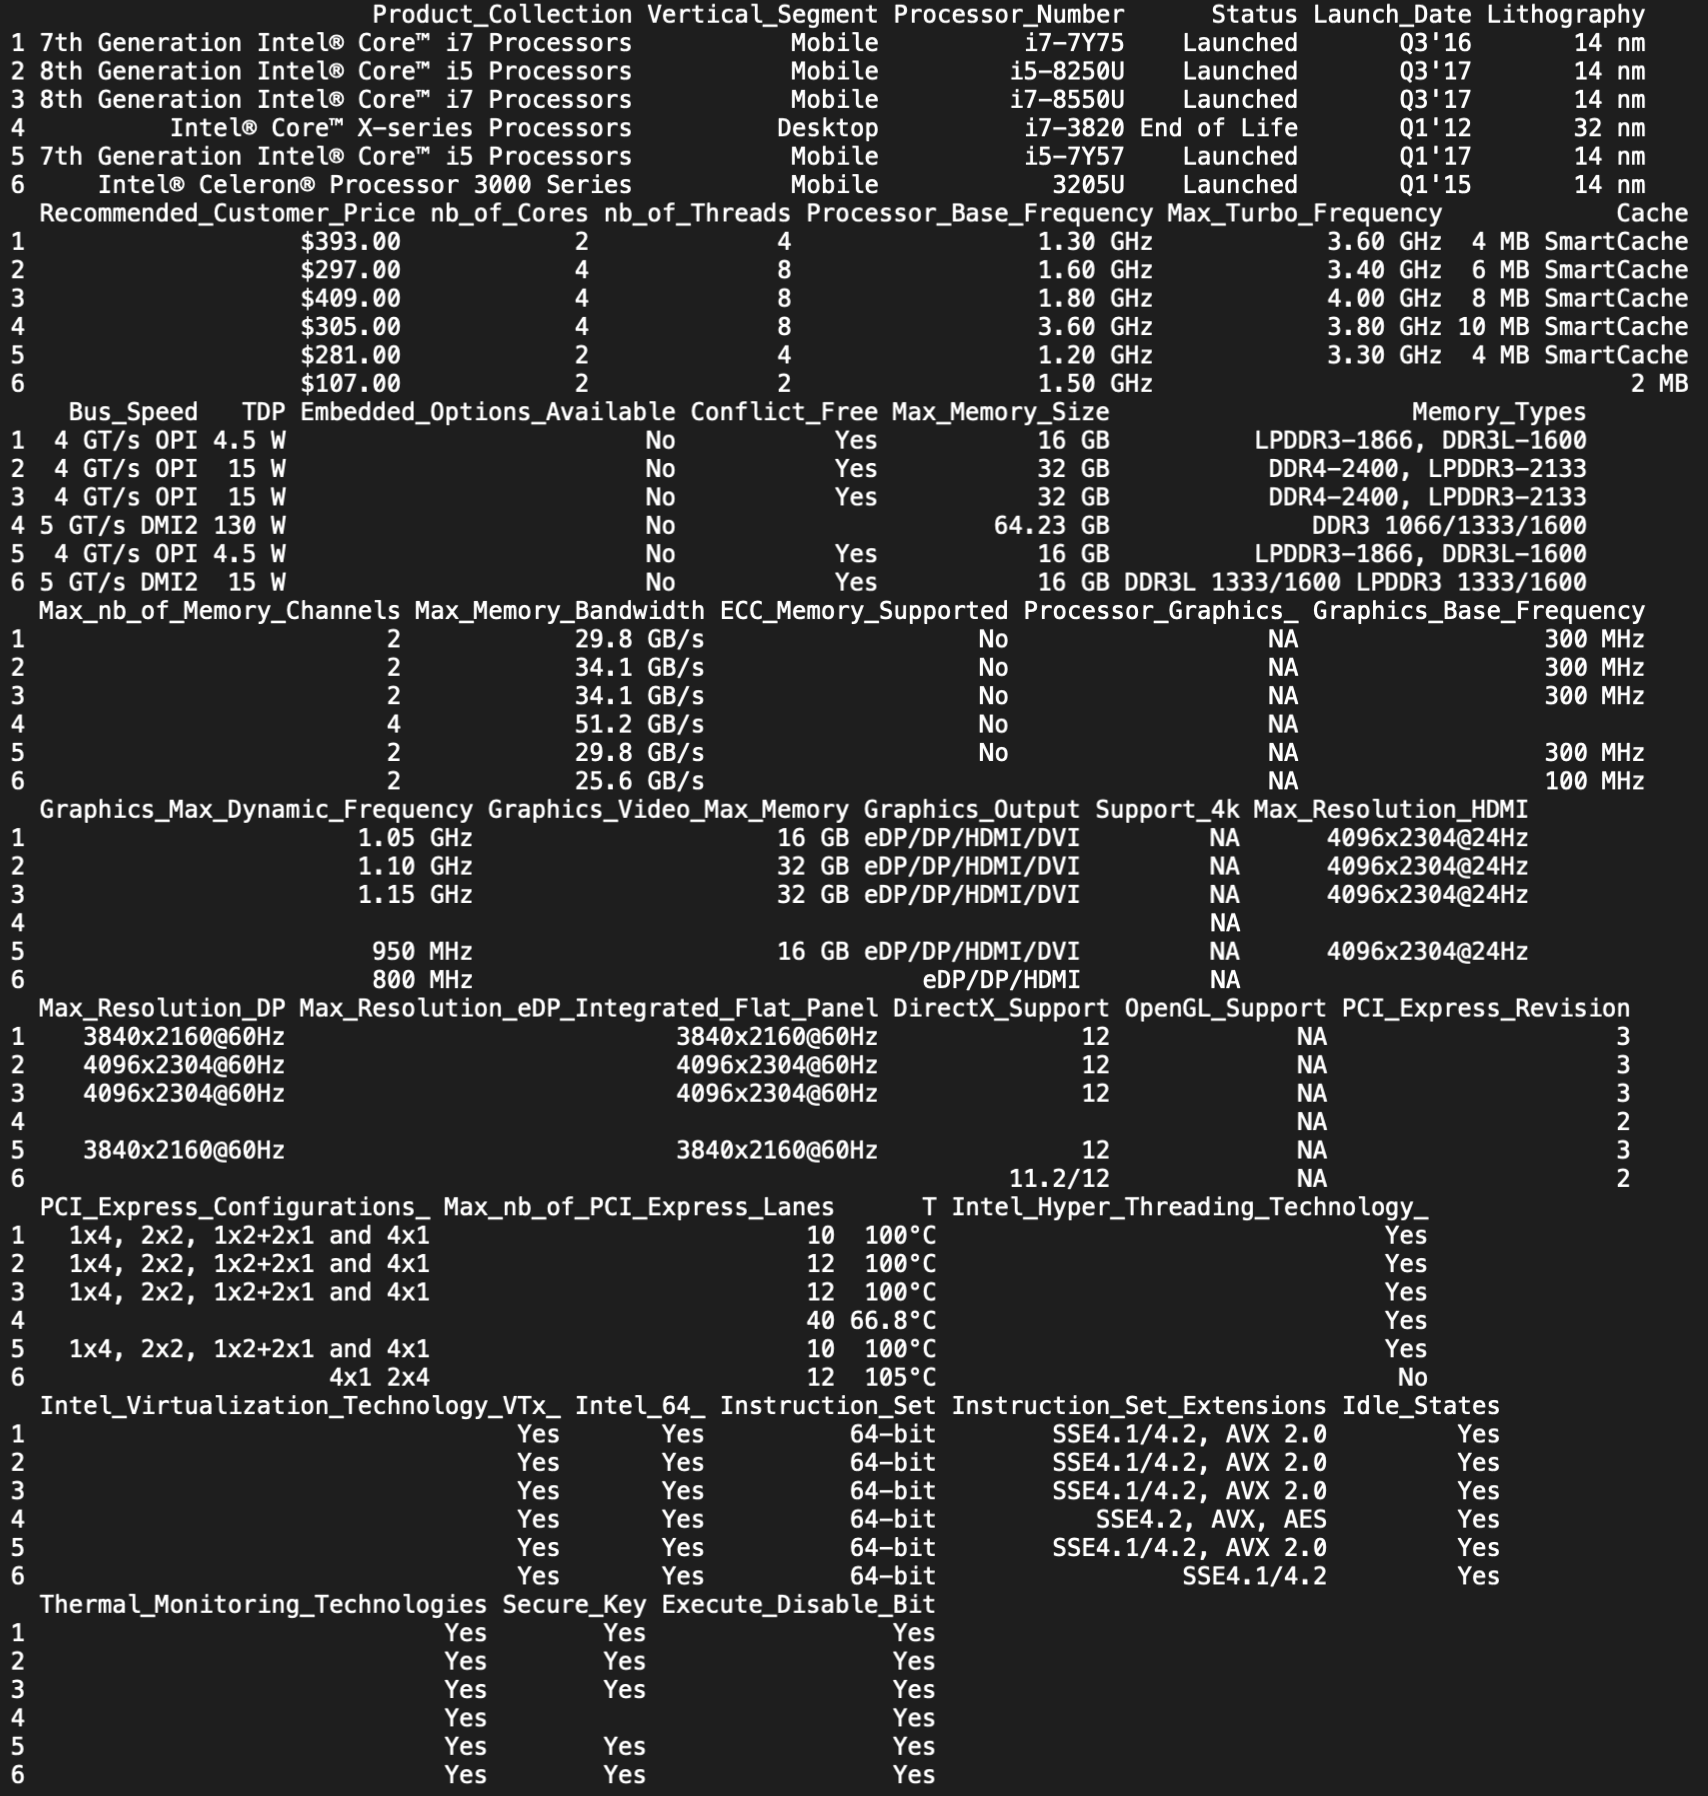
\includegraphics[width=14cm]{graphics/head.png}
    \caption*{Console output of \texttt{head(intel\_cpu)}}
\end{figure}

By executing \texttt{head(intel\_cpu)}, the output will display the first \textit{six} rows of the \texttt{intel\_cpu} data frame, allowing you to visually inspect the data and make informed decisions about the next steps in the data analysis workflow.

\newpage

\begin{lstlisting}[language=R]
    # Summary statistics
    summary (intel_cpu)
\end{lstlisting}

This code snippet is used to obtain summary statistics for the dataset stored in \texttt{intel\_cpu}.\\

The \texttt{summary ()} function in \texttt{R} is a versatile tool that provides a consise summary of the data, depending on the type of input it receives.

\begin{figure}[H]
    \centering
    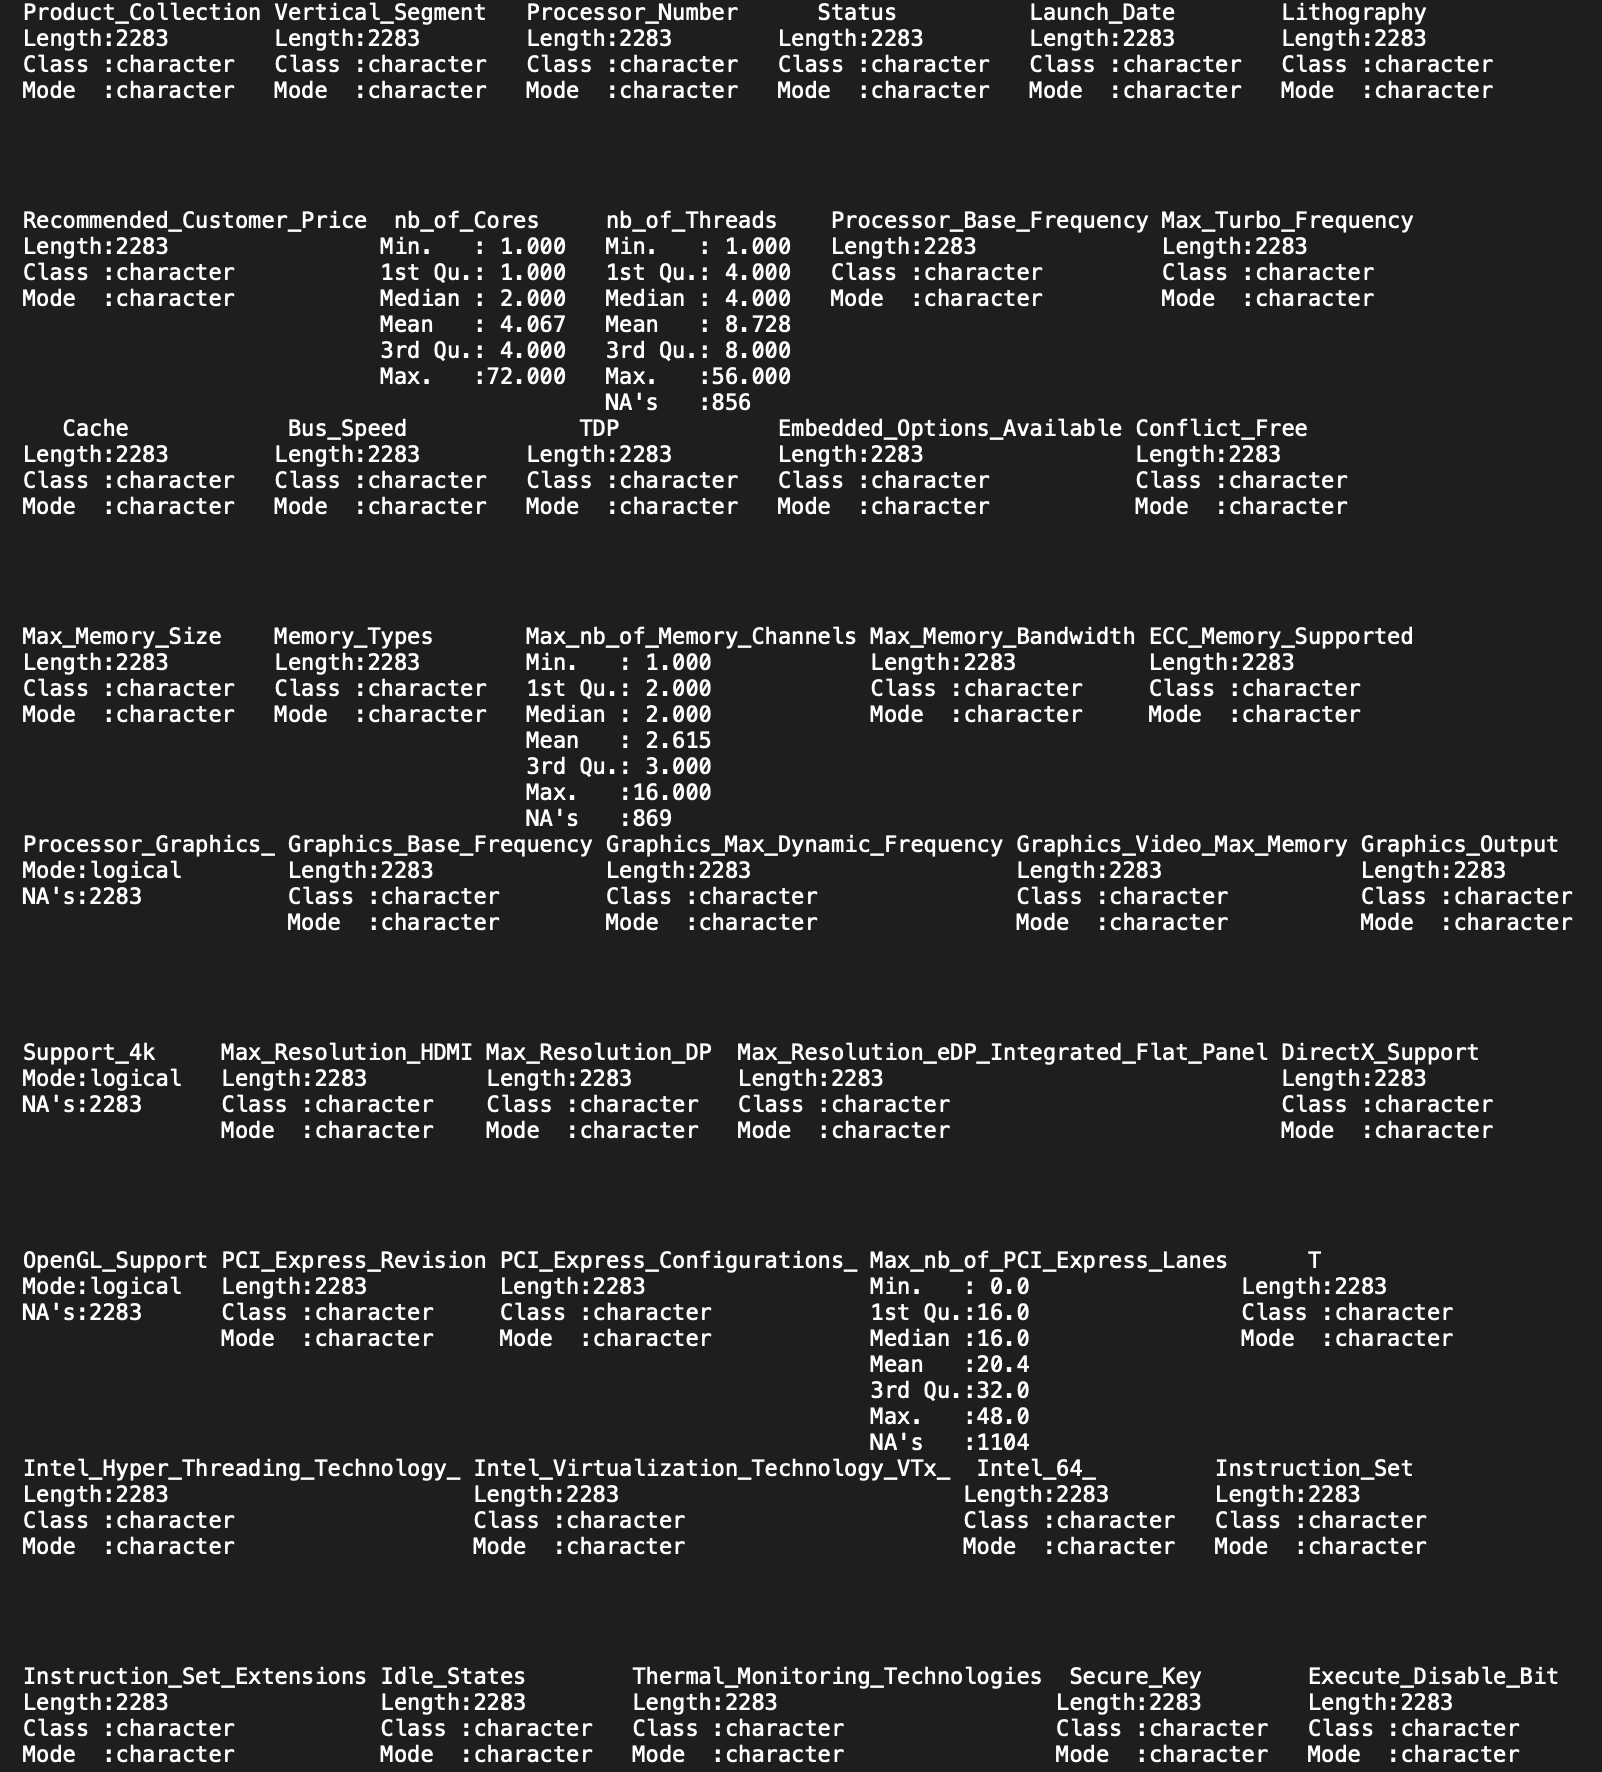
\includegraphics[width=14cm]{graphics/summary.png}
    \caption*{Console output of \texttt{summary(intel\_cpu)}}
\end{figure}

\subsection{Handle Missing Values}

\subsection{Handle Outliers}

\subsection{Feature Scaling/Normalization}

\newpage
% %%%%%%%%%%%%%%%%%%%%%%%%%%%%%%%%%
\section{Conclusion}

\newpage
% %%%%%%%%%%%%%%%%%%%%%%%%%%%%%%%%%
\clearpage
\bibliographystyle{plain}
\bibliography{citations/books.bib}
\nocite{*}

\end{document}